\documentclass[../main/thesis.tex]{subfiles}
\begin{document}

\chapter{Gain Linearity Graphs}
\label{a-gainlin}

\begin{figure} [h!]%2016.07.18 & 2016.08.12
	\centering
	\begin{subfigure}{.5\textwidth}
		\centering
		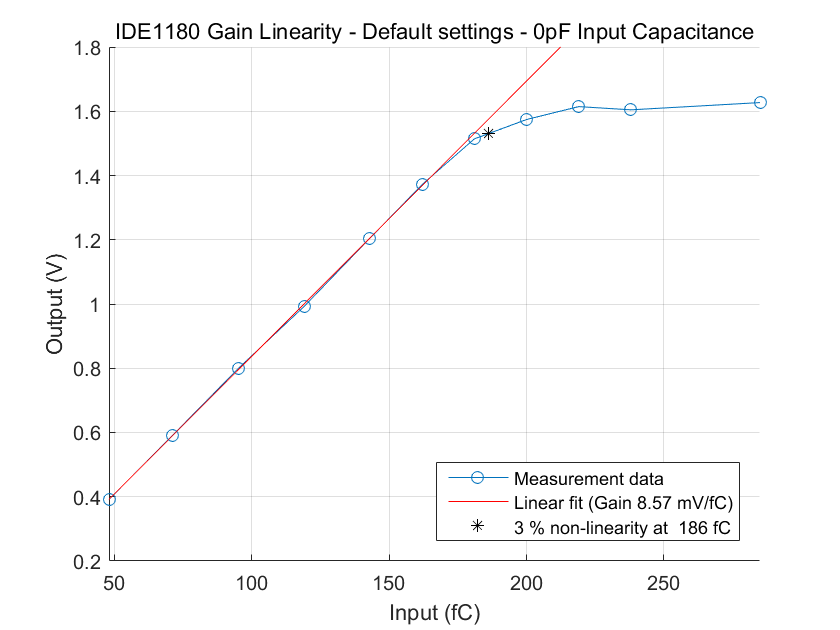
\includegraphics[width=\linewidth]{40ns_0pF.png}
		\caption{0 pF input load capacitance.}
		\label{fig-gainlin-40-0}
	\end{subfigure}%
	\begin{subfigure}{.5\textwidth}
		\centering
		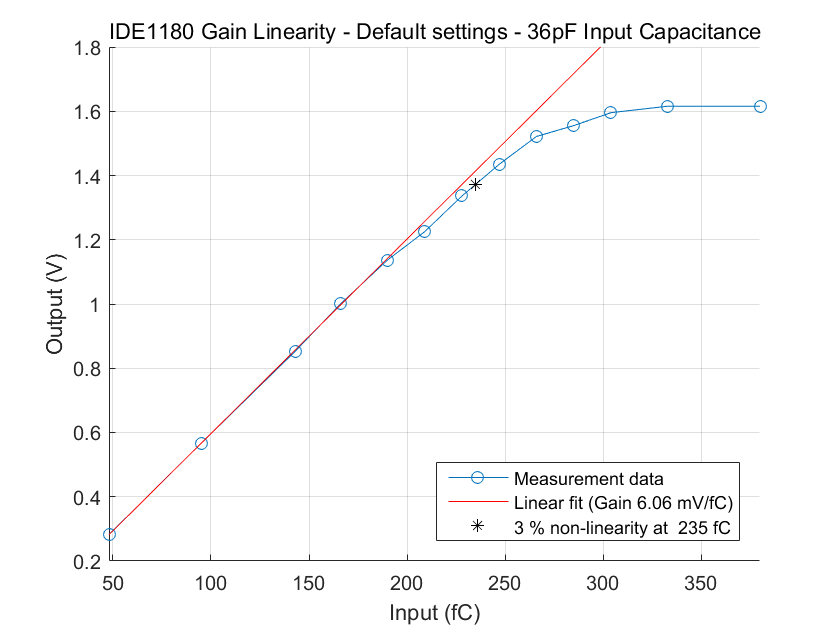
\includegraphics[width=\textwidth]{40ns_33pF.png}
		\caption{33 pF input load capacitance.}
		\label{fig-gainlin-40-33} 
	\end{subfigure}
	\caption{Gain linearity measurements for default settings.}
	\label{fig-gainlin-def}
\end{figure}

\begin{figure} [h!]%2016.07.18 & 2016.08.12
	\centering
	\begin{subfigure}{.5\textwidth}
		\centering
		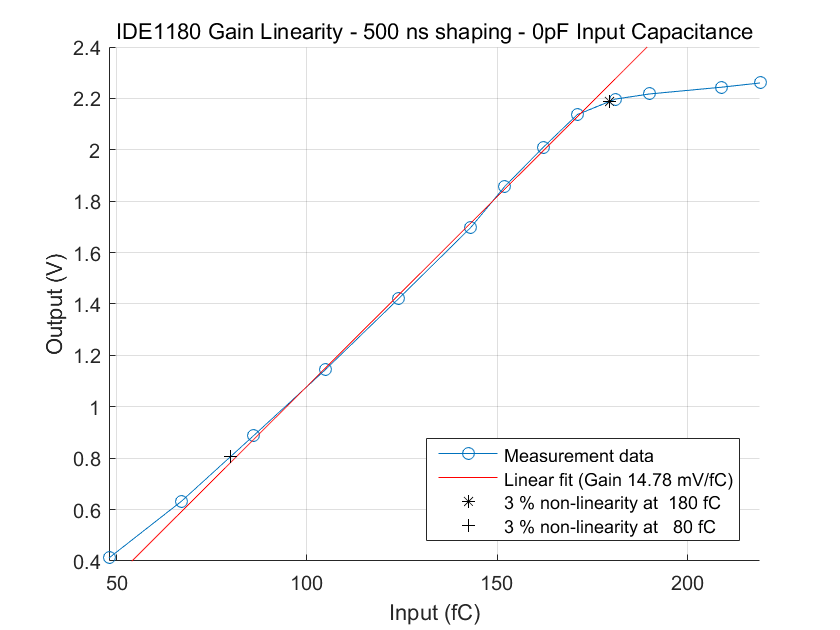
\includegraphics[width=\linewidth]{500ns_0pF.png}
		\caption{0 pF input load capacitance.}
		\label{fig-gainlin-500-0}
	\end{subfigure}%
	\begin{subfigure}{.5\textwidth}
		\centering
		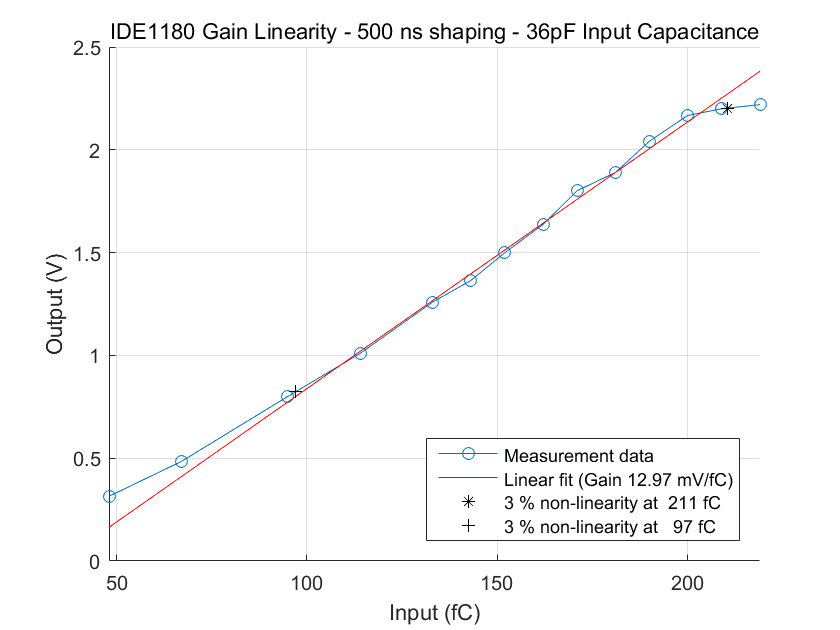
\includegraphics[width=\textwidth]{500ns_33pF.png}
		\caption{33 pF input load capacitance.}
		\label{fig-gainlin-500-33} 
	\end{subfigure}
	\caption{Gain linearity measurements for 500 ns shaping time.}
	\label{fig-gainlin-500}
\end{figure}

\begin{figure} %2016.07.18 & 2016.08.12
	\centering
	\begin{subfigure}{.5\textwidth}
		\centering
		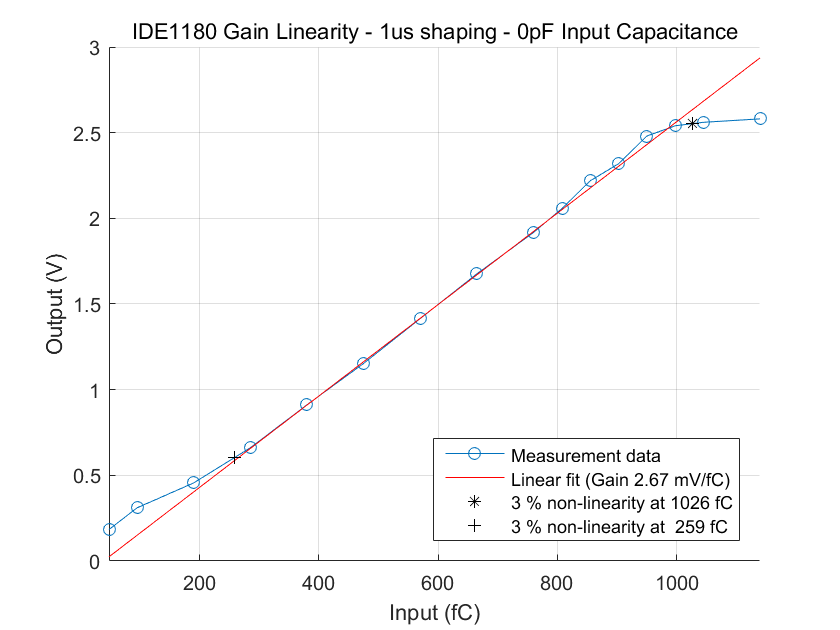
\includegraphics[width=\linewidth]{1us_0pF.png}
		\caption{0 pF input load capacitance.}
		\label{fig-gainlin-1-0}
	\end{subfigure}%
	\begin{subfigure}{.5\textwidth}
		\centering
		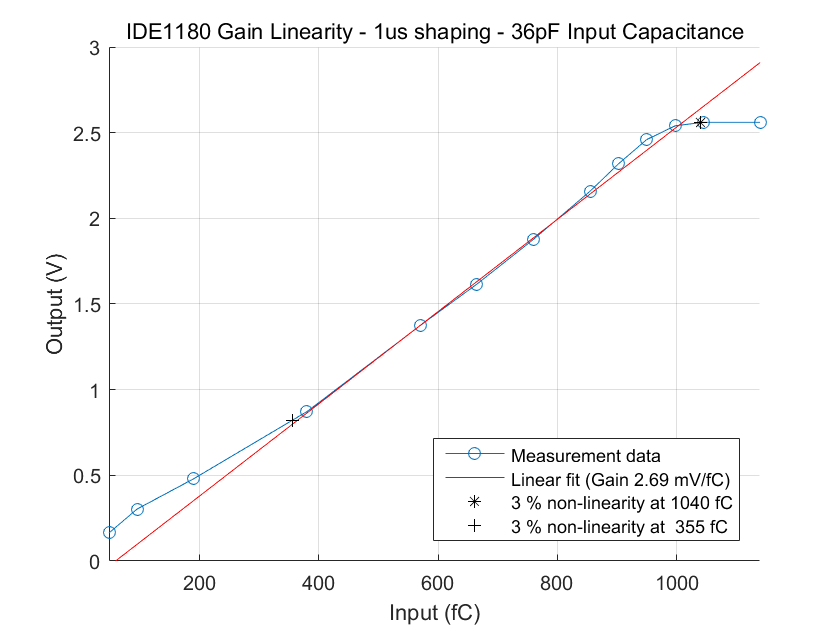
\includegraphics[width=\textwidth]{1us_33pF.png}
		\caption{33 pF input load capacitance.}
		\label{fig-gainlin-1-33} 
	\end{subfigure}
	\caption{Gain linearity measurements for 1 $\mu$s shaping time.}
	\label{fig-gainlin-1}
\end{figure}

\begin{figure} %2016.07.18 & 2016.08.12
	\centering
	\begin{subfigure}{.5\textwidth}
		\centering
		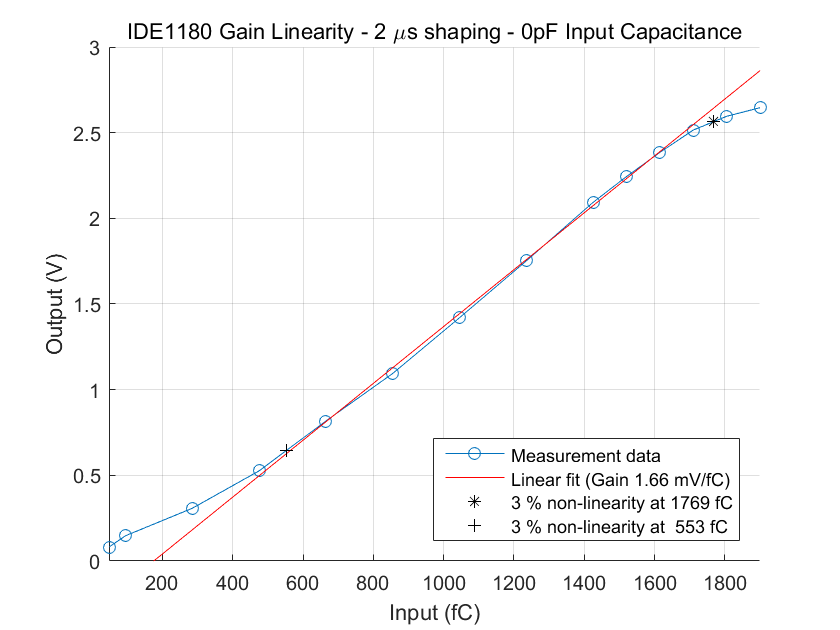
\includegraphics[width=\linewidth]{2us_0pF.png}
		\caption{0 pF input load capacitance.}
		\label{fig-gainlin-2-0}
	\end{subfigure}%
	\begin{subfigure}{.5\textwidth}
		\centering
		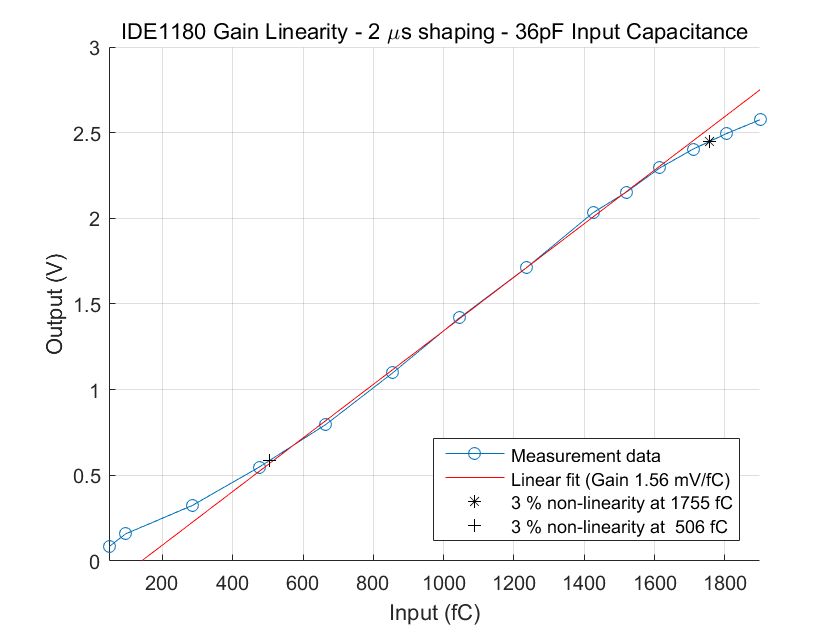
\includegraphics[width=\textwidth]{2us_33pF.png}
		\caption{33 pF input load capacitance.}
		\label{fig-gainlin-2-33} 
	\end{subfigure}
	\caption{Gain linearity measurements for 2 $\mu$s shaping time.}
	\label{fig-gainlin-2}
\end{figure}

\end{document}